% =====================================================================
%  DEFENSE SLIDE DECK (15-20 min), written for a beginner audience
%  Real-Time Financial Fraud Detection with Learned Hybrid Gating and
%  Uncertainty-Aware Triage
%
%  Compile with XeLaTeX (the author names need Ə / ə / ş):
%    Overleaf -> Menu -> Settings -> Compiler -> XeLaTeX
%
%  Figures live in figures/. Regenerate the PDF charts from committed
%  results with:  .venv/Scripts/python presentation/make_figures.py
%  Every number on these slides matches report/main.tex or results/.
%
%  Timing guide (20 slides, ~17 min):
%    Why it matters 3 min | How it works 5 min | Results 7 min |
%    Product + wrap-up 2 min
% =====================================================================
\RequirePackage{fix-cm}
\documentclass[aspectratio=169,11pt]{beamer}

% ---------------------------------------------------------------------
% Packages
% ---------------------------------------------------------------------
\usepackage{fontspec}
\usepackage{amsmath,amssymb}
\usepackage{booktabs}
\usepackage{tikz}
\usetikzlibrary{arrows.meta,positioning,calc,decorations.pathreplacing,fit}
\usefonttheme{professionalfonts}

% Fira Sans when available (Overleaf has it), DejaVu Sans otherwise.
% Fonts are loaded by file name so any TeX Live / Tectonic install finds them.
\IfFontExistsTF{FiraSans-Regular.otf}{%
  \setsansfont{FiraSans}[
    Extension=.otf,
    UprightFont=*-Regular,
    BoldFont=*-SemiBold,
    ItalicFont=*-Italic,
    BoldItalicFont=*-SemiBoldItalic]
}{%
  \setsansfont{DejaVuSans}[
    Extension=.ttf,
    UprightFont=*,
    BoldFont=*-Bold,
    ItalicFont=*-Oblique,
    BoldItalicFont=*-BoldOblique]
}
\newfontfamily\azfont{DejaVuSans}[
  Extension=.ttf,
  UprightFont=*,
  BoldFont=*-Bold]
% Use the main font for Azerbaijani names when it has the glyphs, else DejaVu.
\newcommand{\az}[1]{\iffontchar\font"0259 #1\else{\azfont #1}\fi}

\graphicspath{{figures/}}

% ---------------------------------------------------------------------
% Colors (match report/contribution_report.tex and the figure palette)
% ---------------------------------------------------------------------
\definecolor{brand}{RGB}{24,92,69}
\definecolor{brandmid}{HTML}{4E9A78}
\definecolor{brandlight}{HTML}{E8F2ED}
\definecolor{ink}{HTML}{1F2A2E}
\definecolor{muted}{HTML}{6B7479}
\definecolor{approve}{HTML}{185C45}
\definecolor{review}{HTML}{E3A21A}
\definecolor{block}{HTML}{C0392B}
\definecolor{gatec}{HTML}{3E6FA8}
\definecolor{fraudc}{HTML}{7A3E9D}

% TikZ styles live in the preamble: '#1' inside a frame body breaks \foreach.
\tikzset{
  box/.style={rounded corners=4pt,draw=#1,fill=#1!9,line width=1pt,align=center,
    inner sep=5pt,text=ink},
  box/.default=brand,
  blk/.style={rounded corners=4pt,draw=#1,fill=#1!9,line width=1pt,align=center,
    text=ink,inner sep=4pt},
  blk/.default=brand,
  inp/.style={rounded corners=3pt,draw=#1,fill=#1!9,line width=0.9pt,text width=4.1cm,
    align=left,inner sep=4pt,text=ink},
  inp/.default=muted,
  neuron/.style={circle,minimum size=4.2mm,inner sep=0pt,draw=#1,fill=#1!20,line width=0.8pt},
  neuron/.default=gatec,
  arr/.style={-{Stealth[length=2.3mm]},line width=1pt,draw=muted},
  pill/.style={fill=#1,text=white,rounded corners=3pt,font=\footnotesize\bfseries,
    minimum width=2.2cm,minimum height=0.55cm},
  detail/.style={draw=brandmid,fill=brandmid!12,rounded corners=2pt,minimum width=2.1cm,
    minimum height=0.46cm,font=\scriptsize,text=ink,inner sep=2pt},
  past/.style={draw=review,fill=review!35,rounded corners=2pt,minimum width=0.55cm,
    minimum height=0.46cm,font=\scriptsize\bfseries,text=ink,inner sep=0pt},
}

% ---------------------------------------------------------------------
% Theme
% ---------------------------------------------------------------------
\setbeamertemplate{navigation symbols}{}
\setbeamersize{text margin left=0.9cm,text margin right=0.9cm}

\setbeamercolor{normal text}{fg=ink,bg=white}
\setbeamercolor{structure}{fg=brand}
\setbeamercolor{frametitle}{fg=brand}
\setbeamercolor{kicker}{fg=brandmid}
\setbeamercolor{takeaway}{fg=ink,bg=brandlight}
\setbeamercolor{card}{fg=ink,bg=brandlight}
\setbeamercolor{alerted text}{fg=block}

\setbeamerfont{frametitle}{size=\Large,series=\bfseries}
\setbeamerfont{kicker}{size=\scriptsize,series=\bfseries}

% Thin progress bar across the top of every frame.
\setbeamertemplate{headline}{%
  \begin{tikzpicture}
    \fill[brandlight] (0,0) rectangle (\paperwidth,0.55ex);
    \pgfmathsetmacro{\progressfrac}{min(\insertframenumber/max(\inserttotalframenumber,1),1)}
    \fill[brand] (0,0) rectangle ({\progressfrac*\paperwidth},0.55ex);
  \end{tikzpicture}%
}

% Section kicker above a plain-language frame title.
\setbeamertemplate{frametitle}{%
  \nointerlineskip
  \begin{beamercolorbox}[wd=\paperwidth,sep=0pt,leftskip=0.9cm,rightskip=0.9cm]{frametitle}%
    \vskip0.35em
    {\usebeamerfont{kicker}\usebeamercolor[fg]{kicker}\insertsectionhead\strut}\par
    {\usebeamerfont{frametitle}\insertframetitle\strut\par}%
    \vskip0.1em
  \end{beamercolorbox}%
}

% Slide counter (bottom right).
\setbeamertemplate{footline}{%
  \hbox to \paperwidth{%
    \hfill
    {\scriptsize\color{muted}Fraud Triage Engine\quad
      \textcolor{ink}{\insertframenumber}\,/\,\inserttotalframenumber}%
    \hspace{0.9cm}}%
  \vspace{0.55em}%
}

\setbeamertemplate{itemize items}{\textcolor{brandmid}{\raisebox{0.2ex}{\scriptsize$\blacksquare$}}}
\setlength{\leftmargini}{1.1em}

% ---------------------------------------------------------------------
% Slide helpers
% ---------------------------------------------------------------------
% Big-number callout: [color]{number}{label}
\newcommand{\bignum}[3][brand]{%
  \begin{minipage}[t]{\linewidth}\centering
    {\fontsize{24}{26}\selectfont\bfseries\color{#1}#2}\\[0.35em]
    {\footnotesize\color{muted}#3}
  \end{minipage}}

% Compact number callout for slides that also carry a chart.
\newcommand{\midnum}[3][brand]{%
  \begin{minipage}[t]{\linewidth}\centering
    {\fontsize{19}{21}\selectfont\bfseries\color{#1}#2}\\[0.2em]
    {\scriptsize\color{muted}#3}
  \end{minipage}}

% Short heading + one or two plain sentences.
\newcommand{\point}[2]{%
  {\small\bfseries\color{brand}#1\par}\vspace{0.1em}
  {\footnotesize #2\par}}

% Highlighted conclusion box at the bottom of a slide.
\newcommand{\takeaway}[1]{%
  \par\vspace{0.35em}
  \begin{beamercolorbox}[wd=\linewidth,sep=0.45em,rounded=true]{takeaway}%
    \small #1
  \end{beamercolorbox}}

% One-line variant for dense slides.
\newcommand{\keyline}[1]{%
  \par\vspace{0.25em}
  \begin{beamercolorbox}[wd=\linewidth,sep=0.35em,rounded=true]{takeaway}%
    \footnotesize #1
  \end{beamercolorbox}}

% Small provenance line.
\newcommand{\source}[1]{\par\vspace{0.15em}{\tiny\color{muted}#1}}

% Colored pill: {color}{text}
\newcommand{\chip}[2]{%
  \tikz[baseline=(c.base)]\node[fill=#1,text=white,rounded corners=2.5pt,
    inner xsep=4pt,inner ysep=2.5pt,font=\scriptsize\bfseries](c){#2};}

% Screenshot with a thin frame; dashed placeholder if the file is missing.
\newcommand{\screenshot}[3]{% {file}{width}{placeholder label}
  \IfFileExists{figures/#1}{%
    \tikz\node[inner sep=0pt,draw=black!18,line width=0.6pt]{\includegraphics[width=#2]{#1}};%
  }{%
    \tikz\node[draw=muted,dashed,rounded corners=3pt,minimum width=#2,
      minimum height={0.5625*#2},font=\footnotesize,text=muted,align=center]{#3};%
  }}

% Card for the "three challenges" slide.
\newcommand{\gapcard}[4]{% {challenge}{why it hurts}{our idea}{how}
  \begin{beamercolorbox}[wd=\linewidth,sep=0.5em,rounded=true]{card}
    {\small\bfseries\color{block}#1\par}\vspace{0.2em}
    {\footnotesize #2\par}\vspace{0.2em}
    {\centering\color{brandmid}$\Downarrow$\par}\vspace{0.1em}
    {\small\bfseries\color{brand}#3\par}\vspace{0.1em}
    {\footnotesize #4\par}
  \end{beamercolorbox}}

% Speaker names (from report/contribution_report.tex)
\newcommand{\sNadir}{\az{Nadir Əskərov}}
\newcommand{\sAkshin}{\az{Akşin Fətəliyev}}
\newcommand{\sSebuhi}{\az{Səbuhi Nəzərov}}
\newcommand{\sHabil}{\az{Habil Hüseynov}}
\newcommand{\sAll}{All members}
\newcommand{\speaker}[1]{\par\vspace{-0.9em}\hfill{\scriptsize\color{muted}#1}\par\vspace{-0.2em}}

\title{Real-Time Financial Fraud Detection}
\subtitle{Catching rare fraud with deep learning, and knowing when to ask a human}

% =====================================================================
\begin{document}
% =====================================================================

% ---------------------------------------------------------------------
% 1. Title
% ---------------------------------------------------------------------
{
\setbeamertemplate{headline}{}
\setbeamertemplate{footline}{}
\begin{frame}[plain]
  \begin{tikzpicture}[remember picture,overlay]
    \fill[brand] (current page.north west) rectangle ([xshift=0.42cm]current page.south west);
    \node[anchor=south east,align=right] at ([xshift=-0.9cm,yshift=0.85cm]current page.south east)
      {\chip{approve}{APPROVE}\ \chip{review}{REVIEW}\ \chip{block}{BLOCK}};
  \end{tikzpicture}
  \vspace*{0.9cm}
  {\scriptsize\bfseries\color{brandmid}DEEP LEARNING FINAL PROJECT\enspace\textperiodcentered\enspace TRACK 3: INDUSTRY PRODUCT}\par
  \vspace{0.7em}
  {\fontsize{22}{26}\selectfont\bfseries\color{brand}\inserttitle}\par
  \vspace{0.3em}
  {\large\color{ink}\insertsubtitle}\par
  \vspace{0.9em}
  {\color{brandmid}\rule{0.5\linewidth}{1.2pt}}\par
  \vspace{0.9em}
  {\normalsize \sNadir\enspace\textperiodcentered\enspace \sAkshin\enspace\textperiodcentered\enspace
    \sHabil\enspace\textperiodcentered\enspace \sSebuhi}\par
  \vspace{0.35em}
  {\footnotesize\color{muted}AI Academy, National Artificial Intelligence Center, Azerbaijan\enspace\textperiodcentered\enspace DLE-AI-202}\par
  \vfill
  {\footnotesize\color{muted}github.com/sa6uhi/DL-final-project}\par
  \vspace{0.55cm}
\end{frame}
}

% =====================================================================
\section{Why it matters}
% =====================================================================

% ---------------------------------------------------------------------
% 2. Why fraud detection is hard
% ---------------------------------------------------------------------
\speaker{\sNadir}
\begin{frame}{Why is fraud detection hard?}
  \vspace{0.2em}
  \begin{columns}[T]
    \column{0.31\textwidth}
      \bignum[block]{1 in 29}{online payments in our data\\is fraud (3.5\%)}
    \column{0.31\textwidth}
      \bignum[review]{96.5\%}{accuracy of a useless model\\that \emph{never} flags fraud}
    \column{0.31\textwidth}
      \bignum{3 choices}{for every payment: approve,\\block, or ask a human}
  \end{columns}
  \vspace{1.1em}
  \begin{columns}[T]
    \column{0.31\textwidth}
      \point{Fraud is rare}{Models see very few fraud examples to learn from.}
    \column{0.31\textwidth}
      \point{Fraud changes}{Criminals keep inventing tricks the model has never seen.}
    \column{0.31\textwidth}
      \point{Mistakes are costly}{Missed fraud loses money; false alarms annoy real customers.}
  \end{columns}
  \vfill
  \takeaway{Our goal: a fast system that spots fraud \textbf{and knows when it is unsure},
    so only the difficult cases go to a human analyst.}
\end{frame}

% ---------------------------------------------------------------------
% 3. Three challenges, three ideas
% ---------------------------------------------------------------------
\speaker{\sNadir}
\begin{frame}{Three challenges, three ideas}
  \begin{columns}[T]
    \column{0.31\textwidth}
      \gapcard{1\enspace Single payments}
        {Looking at one payment alone misses patterns, like many purchases in a few minutes.}
        {Transformer with history}
        {Looks at the payment \emph{and} at the card's last 5 payments.}
    \column{0.31\textwidth}
      \gapcard{2\enspace New fraud tricks}
        {A model trained on past fraud can miss a trick it has never seen.}
        {Autoencoder}
        {Learns what \emph{normal} payments look like and flags anything unusual.}
    \column{0.31\textwidth}
      \gapcard{3\enspace No confidence}
        {A score of 0.6 does not tell us whether we can trust it.}
        {Confidence check}
        {Acts automatically only when sure; otherwise asks a human.}
  \end{columns}
  \vfill
  \keyline{A small \textbf{gate} combines the two detectors, and everything runs as a web
    service with an analyst dashboard.}
\end{frame}

% ---------------------------------------------------------------------
% 4. Data and time split
% ---------------------------------------------------------------------
\speaker{\sNadir}
\begin{frame}{The data: real payments, split by time}
  \vspace{0.1em}
  \begin{columns}[T]
    \column{0.31\textwidth}\midnum{590,540}{real online payments (IEEE-CIS / Vesta)}
    \column{0.31\textwidth}\midnum{≈430}{details per payment: amount, card, email, device…}
    \column{0.31\textwidth}\midnum[block]{20,663}{payments labelled as fraud}
  \end{columns}
  \vspace{0.5em}
  \centering
  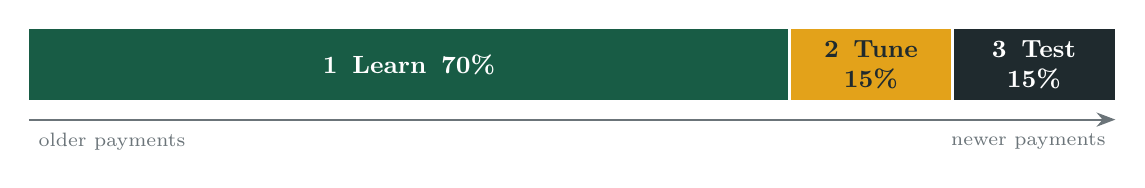
\begin{tikzpicture}[x=0.138cm,y=1cm]
    \def\h{0.9}
    \fill[brand]  (0,0)  rectangle (70,\h);
    \fill[review] (70,0) rectangle (85,\h);
    \fill[ink]    (85,0) rectangle (100,\h);
    \draw[white,line width=1pt] (70,0) -- (70,\h) (85,0) -- (85,\h);
    \node[white,font=\small\bfseries] at (35,\h/2) {1\enspace Learn\enspace 70\%};
    \node[ink,font=\small\bfseries,align=center] at (77.5,\h/2) {2\enspace Tune\\15\%};
    \node[white,font=\small\bfseries,align=center] at (92.5,\h/2) {3\enspace Test\\15\%};
    \draw[muted,-{Stealth[length=2.4mm]},thick] (0,-0.25) -- (100,-0.25);
    \node[font=\scriptsize,text=muted,anchor=north west] at (0,-0.3) {older payments};
    \node[font=\scriptsize,text=muted,anchor=north east] at (100,-0.3) {newer payments};
  \end{tikzpicture}
  \vspace{0.3em}
  \raggedright
  \begin{columns}[T]
    \column{0.31\textwidth}
      \point{1\enspace Learn}{The two detectors learn from the oldest 70\% of payments.}
    \column{0.31\textwidth}
      \point{2\enspace Tune}{The next 15\% trains the gate and sets the cut-off.}
    \column{0.31\textwidth}
      \point{3\enspace Test}{The newest 15\% (88,581 payments) is kept for the end.}
  \end{columns}
  \vfill
  \keyline{Like studying old exams, then sitting a new one: the models never see the future.}
\end{frame}

% ---------------------------------------------------------------------
% 5. How we measure success
% ---------------------------------------------------------------------
\speaker{\sNadir}
\begin{frame}{How do we measure success?}
  \vspace{0.2em}
  \begin{columns}[T]
    \column{0.31\textwidth}
      \begin{beamercolorbox}[wd=\linewidth,sep=0.5em,rounded=true]{card}
        \point{Accuracy can fool us}{Saying ``normal'' for every payment is 96.5\% accurate,
          but catches no fraud at all.}
      \end{beamercolorbox}
    \column{0.31\textwidth}
      \begin{beamercolorbox}[wd=\linewidth,sep=0.5em,rounded=true]{card}
        \point{Precision}{Of the payments we flag, how many are \emph{really} fraud?}
      \end{beamercolorbox}
    \column{0.31\textwidth}
      \begin{beamercolorbox}[wd=\linewidth,sep=0.5em,rounded=true]{card}
        \point{Recall}{Of all the real fraud, how much did we \emph{catch}?}
      \end{beamercolorbox}
  \end{columns}
  \vspace{1.0em}
  \centering
  {\small\textbf{\color{brand}PR-AUC} combines precision and recall into one score from 0 to 1}\par
  \vspace{1.5em}
  \begin{tikzpicture}[x=12cm,y=1cm]
    \fill[brandlight] (0,0) rectangle (1,0.4);
    \fill[brandmid!55] (0.33,0) rectangle (0.52,0.4);
    \draw[muted] (0,0) rectangle (1,0.4);
    \foreach \v in {0,0.25,0.5,0.75,1} \node[below,font=\scriptsize,text=muted] at (\v,0) {\v};
    \draw[block,line width=1.6pt] (0.035,-0.08) -- (0.035,0.55);
    \node[anchor=south west,font=\scriptsize\bfseries,text=block] at (0,0.58) {random guessing ≈ 0.035};
    \node[anchor=south,font=\scriptsize\bfseries,text=brand] at (0.425,0.58) {our models ≈ 0.33--0.52};
    \draw[approve,line width=1.6pt] (1,-0.08) -- (1,0.55);
    \node[anchor=south east,font=\scriptsize\bfseries,text=approve] at (1,0.58) {perfect = 1};
  \end{tikzpicture}
  \vfill
  \raggedright
  \keyline{We also report how much fraud is caught when only 1 in 100 normal payments
    is wrongly flagged.}
\end{frame}

% =====================================================================
\section{How it works}
% =====================================================================

% ---------------------------------------------------------------------
% 6. System in one picture
% ---------------------------------------------------------------------
\speaker{\sSebuhi}
\begin{frame}{Our system in one picture}
  \vspace{0.4em}
  \centering
  \resizebox{\linewidth}{!}{%
  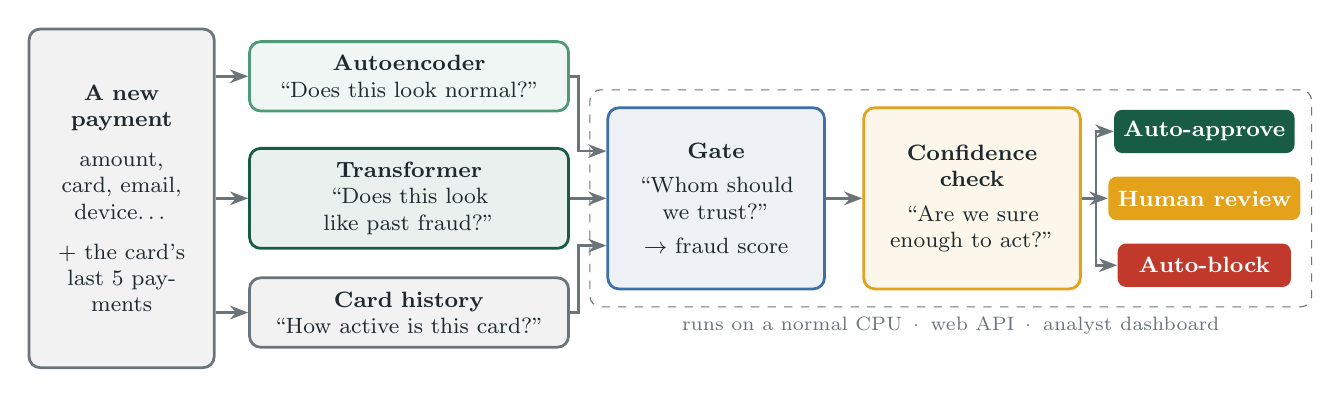
\begin{tikzpicture}[font=\footnotesize]
    \node[box=muted,text width=2.0cm,minimum height=4.3cm] (in) at (0,0)
      {\textbf{A new payment}\\[5pt]amount, card, email, device…\\[5pt]+ the card's last 5 payments};

    \node[box=brandmid,text width=3.7cm] (dae) at (3.65,1.55)
      {\textbf{Autoencoder}\\``Does this look normal?''};
    \node[box=brand,text width=3.7cm] (ft) at (3.65,0)
      {\textbf{Transformer}\\``Does this look like past fraud?''};
    \node[box=muted,text width=3.7cm] (hist) at (3.65,-1.45)
      {\textbf{Card history}\\``How active is this card?''};

    \node[box=gatec,text width=2.4cm,minimum height=2.3cm] (gate) at (7.55,0)
      {\textbf{Gate}\\[3pt]``Whom should we trust?''\\[3pt]$\rightarrow$ fraud score};
    \node[box=review,text width=2.4cm,minimum height=2.3cm] (cp) at (10.8,0)
      {\textbf{Confidence check}\\[3pt]``Are we sure enough to act?''};

    \node[pill=approve] (ap) at (13.75,0.85) {Auto-approve};
    \node[pill=review]  (rv) at (13.75,0)    {Human review};
    \node[pill=block]   (bl) at (13.75,-0.85) {Auto-block};

    \draw[arr] (in.east |- dae.west) -- (dae.west);
    \draw[arr] (in.east |- ft.west) -- (ft.west);
    \draw[arr] (in.east |- hist.west) -- (hist.west);
    \draw[arr] (dae.east) -| ($(gate.west)+(-0.35,0.6)$) -- ($(gate.west)+(0,0.6)$);
    \draw[arr] (ft.east) -- (gate.west);
    \draw[arr] (hist.east) -| ($(gate.west)+(-0.35,-0.6)$) -- ($(gate.west)+(0,-0.6)$);
    \draw[arr] (gate.east) -- (cp.west);
    \draw[arr] (cp.east) -- ++(0.18,0) |- (ap.west);
    \draw[arr] (cp.east) -- (rv.west);
    \draw[arr] (cp.east) -- ++(0.18,0) |- (bl.west);

    \node[draw=muted,dashed,rounded corners=4pt,fit=(gate)(cp)(ap)(bl),inner sep=6pt,
      label={[font=\scriptsize,text=muted]below:runs on a normal CPU\enspace\textperiodcentered\enspace web API\enspace\textperiodcentered\enspace analyst dashboard}] {};
  \end{tikzpicture}}
  \vfill
  \takeaway{Think of two detectives with different skills: one knows \emph{normal} behaviour,
    the other knows \emph{past fraud}. The gate weighs their opinions, and the confidence
    check decides whether to act or ask a human.}
\end{frame}

% ---------------------------------------------------------------------
% 7. Transformer
% ---------------------------------------------------------------------
\speaker{\sAkshin}
\begin{frame}{The Transformer: reading a payment like a sentence}
  \vspace{0.2em}
  \centering
  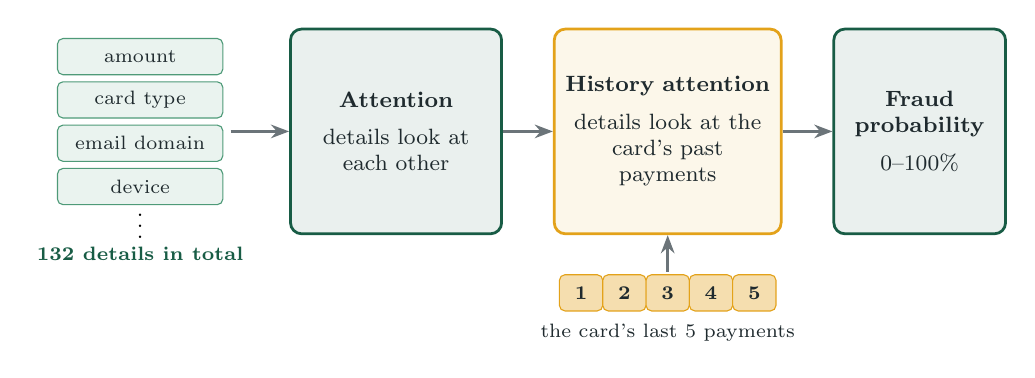
\begin{tikzpicture}[font=\footnotesize]
    \node[detail] (d1) at (0, 1.05) {amount};
    \node[detail] (d2) at (0, 0.5)  {card type};
    \node[detail] (d3) at (0,-0.05) {email domain};
    \node[detail] (d4) at (0,-0.6)  {device};
    \node[font=\footnotesize] at (0,-1.0) {$\vdots$};
    \node[font=\scriptsize\bfseries,text=brand] at (0,-1.45) {132 details in total};

    \node[blk=brand,text width=2.4cm,minimum height=2.6cm] (att) at (3.25,0.1)
      {\textbf{Attention}\\[4pt]details look at\\each other};
    \node[blk=review,text width=2.6cm,minimum height=2.6cm] (hat) at (6.7,0.1)
      {\textbf{History attention}\\[4pt]details look at the\\card's past payments};
    \node[blk=brand,text width=1.9cm,minimum height=2.6cm] (out) at (9.9,0.1)
      {\textbf{Fraud\\probability}\\[4pt]0--100\%};

    \foreach \k in {1,...,5} \node[past] at ({5.6+(\k-1)*0.55},-1.95) {\k};
    \node[font=\scriptsize,text=ink] at (6.7,-2.45) {the card's last 5 payments};

    \draw[arr] (1.15,0.1) -- (att.west);
    \draw[arr] (att.east) -- (hat.west);
    \draw[arr] (hat.east) -- (out.west);
    \draw[arr] (6.7,-1.68) -- (hat.south);
  \end{tikzpicture}
  \vspace{0.3em}
  \raggedright
  \begin{columns}[T]
    \column{0.31\textwidth}
      \point{Like words in a sentence}{Each detail becomes a token, the way a language model
        splits text into words.}
    \column{0.31\textwidth}
      \point{Attention}{The model learns which details matter together, and which past
        payments matter for this one.}
    \column{0.31\textwidth}
      \point{Learning from rare fraud}{Focal loss makes rare, hard fraud examples count more.
        Size: 94k parameters.}
  \end{columns}
\end{frame}

% ---------------------------------------------------------------------
% 8. Autoencoder
% ---------------------------------------------------------------------
\speaker{\sSebuhi}
\begin{frame}{The autoencoder: learning what ``normal'' looks like}
  \vspace{0.4em}
  \begin{columns}[c]
    \column{0.55\textwidth}
      \centering
      \resizebox{\linewidth}{!}{%
      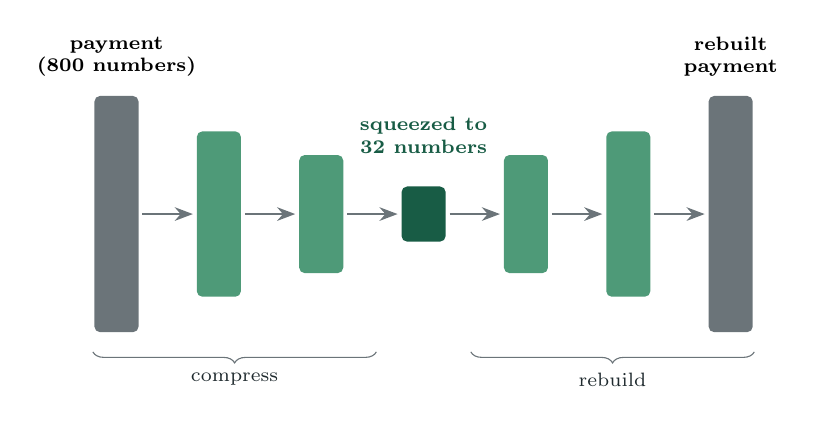
\begin{tikzpicture}[font=\footnotesize]
        \foreach \x/\hh/\col in {0/3.0/muted,1.3/2.1/brandmid,2.6/1.5/brandmid,3.9/0.7/brand,
                                 5.2/1.5/brandmid,6.5/2.1/brandmid,7.8/3.0/muted}
          \fill[\col,rounded corners=2pt] ({\x-0.28},{-\hh/2}) rectangle ({\x+0.28},{\hh/2});
        \foreach \a/\b in {0/1.3,1.3/2.6,2.6/3.9,3.9/5.2,5.2/6.5,6.5/7.8}
          \draw[arr,line width=0.8pt] ({\a+0.33},0) -- ({\b-0.33},0);
        \node[align=center,font=\scriptsize\bfseries] at (0,2.0) {payment\\(800 numbers)};
        \node[align=center,font=\scriptsize\bfseries,text=brand] at (3.9,1.0) {squeezed to\\32 numbers};
        \node[align=center,font=\scriptsize\bfseries] at (7.8,2.0) {rebuilt\\payment};
        \draw[decorate,decoration={brace,amplitude=4pt,mirror},muted] (-0.3,-1.75) -- (3.3,-1.75)
          node[midway,below=4pt,font=\scriptsize,text=ink] {compress};
        \draw[decorate,decoration={brace,amplitude=4pt,mirror},muted] (4.5,-1.75) -- (8.1,-1.75)
          node[midway,below=4pt,font=\scriptsize,text=ink] {rebuild};
      \end{tikzpicture}}
      \vspace{0.6em}
      \begin{beamercolorbox}[wd=\linewidth,sep=0.45em,rounded=true]{takeaway}
        \centering\small
        \textbf{Anomaly score} = how different the rebuilt payment is from the original
      \end{beamercolorbox}
    \column{0.42\textwidth}
      \point{Trained only on normal payments}{It practises squeezing normal payments into
        32 numbers and rebuilding them.}
      \vspace{0.5em}
      {\footnotesize\textcolor{approve}{\textbf{Normal}} $\rightarrow$ rebuilt well
        $\rightarrow$ low score\par}
      \vspace{0.25em}
      {\footnotesize\textcolor{block}{\textbf{Unusual}} $\rightarrow$ rebuilt badly
        $\rightarrow$ high score\par}
      \vspace{0.6em}
      \point{Why ``denoising''?}{We add a little random noise during training, so it learns
        real patterns instead of simply copying.}
      \vspace{0.5em}
      \point{Why is it useful?}{It can flag new fraud tricks that nobody has labelled yet.}
  \end{columns}
\end{frame}

% ---------------------------------------------------------------------
% 9. Gate
% ---------------------------------------------------------------------
\speaker{\sHabil}
\begin{frame}{The gate: deciding which signal to trust}
  \vspace{0.5em}
  \begin{columns}[c]
    \column{0.57\textwidth}
      \centering
      \resizebox{\linewidth}{!}{%
      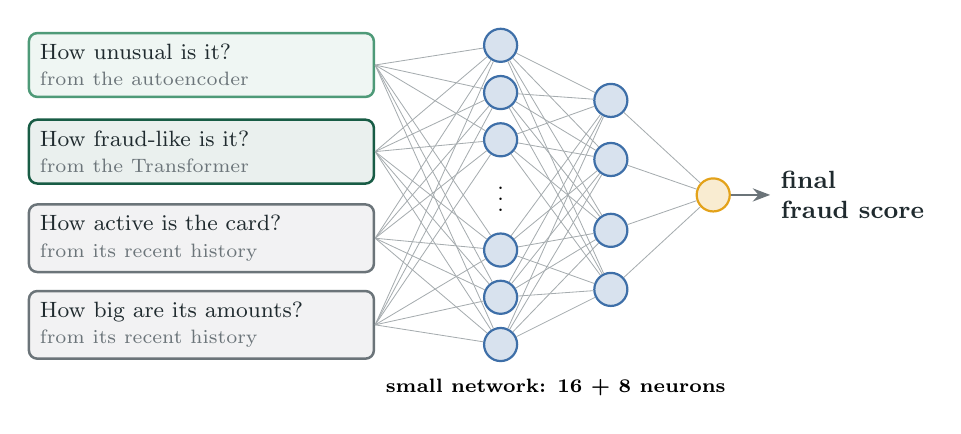
\begin{tikzpicture}[font=\footnotesize]
        \node[inp=brandmid] (i1) at (0, 1.65) {How unusual is it?\\{\scriptsize\color{muted}from the autoencoder}};
        \node[inp=brand]    (i2) at (0, 0.55) {How fraud-like is it?\\{\scriptsize\color{muted}from the Transformer}};
        \node[inp=muted]    (i3) at (0,-0.55) {How active is the card?\\{\scriptsize\color{muted}from its recent history}};
        \node[inp=muted]    (i4) at (0,-1.65) {How big are its amounts?\\{\scriptsize\color{muted}from its recent history}};

        \foreach \j/\y in {1/1.9,2/1.3,3/0.7,4/-0.7,5/-1.3,6/-1.9} \node[neuron] (a\j) at (3.8,\y) {};
        \node at (3.8,0.05) {$\vdots$};
        \foreach \j/\y in {1/1.2,2/0.45,3/-0.45,4/-1.2} \node[neuron] (b\j) at (5.2,\y) {};
        \node[neuron=review] (o) at (6.5,0) {};

        \foreach \i in {1,...,4} \foreach \j in {1,...,6} \draw[muted!60,line width=0.3pt] (i\i.east) -- (a\j);
        \foreach \i in {1,...,6} \foreach \j in {1,...,4} \draw[muted!60,line width=0.3pt] (a\i) -- (b\j);
        \foreach \j in {1,...,4} \draw[muted!60,line width=0.3pt] (b\j) -- (o);

        \node[font=\scriptsize\bfseries] at (4.5,-2.45) {small network: 16 + 8 neurons};
        \draw[-{Stealth[length=2.2mm]},line width=1pt,muted] (o.east) -- ++(0.5,0)
          node[right,text=ink,font=\small\bfseries,align=left] {final\\fraud score};
      \end{tikzpicture}}
    \column{0.40\textwidth}
      \point{Why not a fixed 50/50 mix?}{A fixed mix treats every payment the same way.
        A learned gate can weigh the signals differently in different situations.}
      \vspace{0.6em}
      \point{No cheating}{It is trained on a later time period than the two detectors,
        so it never sees their training data.}
      \vspace{0.6em}
      \point{Tiny and fast}{Only 225 parameters, and about 0.12 ms per payment.}
  \end{columns}
\end{frame}

% ---------------------------------------------------------------------
% 10. Confidence check (conformal prediction)
% ---------------------------------------------------------------------
\speaker{\sHabil}
\begin{frame}{The confidence check: act only when we are sure}
  \vspace{0.2em}
  \begin{columns}[c]
    \column{0.36\textwidth}
      \point{1\enspace Hold out fresh payments}{44,291 payments the models never learned from.}
      \vspace{0.45em}
      \point{2\enspace Measure the mistakes}{Check how wrong the fraud score can be on them.}
      \vspace{0.45em}
      \point{3\enspace Set a safety cut-off}{Chosen so the right answer is covered 99\% of
        the time.}
      \vspace{0.6em}
      {\footnotesize Sure it is normal\hfill\chip{approve}{Auto-approve}\par}
      \vspace{0.25em}
      {\footnotesize Sure it is fraud\hfill\chip{block}{Auto-block}\par}
      \vspace{0.25em}
      {\footnotesize Not sure\hfill\chip{review}{Human review}\par}
      \vspace{0.5em}
      {\scriptsize\color{muted}This method is called \emph{conformal prediction}.\par}
    \column{0.62\textwidth}
      \centering
      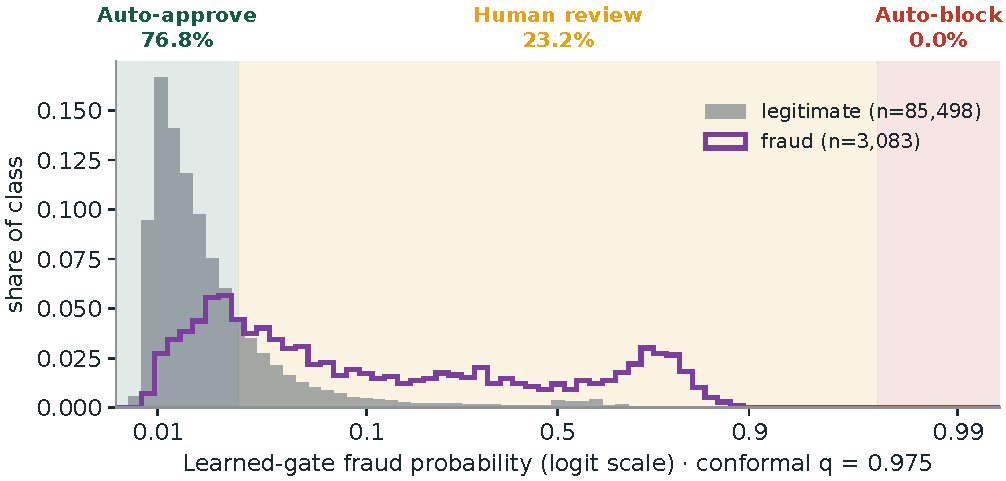
\includegraphics[width=\linewidth]{score_bands.pdf}
      \source{Most normal payments get a very low fraud score.}
  \end{columns}
\end{frame}

% =====================================================================
\section{Results}
% =====================================================================

% ---------------------------------------------------------------------
% 11. Classic baselines
% ---------------------------------------------------------------------
\speaker{\sNadir}
\begin{frame}{Classic models set a strong benchmark}
  \vspace{0.3em}
  \begin{columns}[c]
    \column{0.58\textwidth}
      \centering
      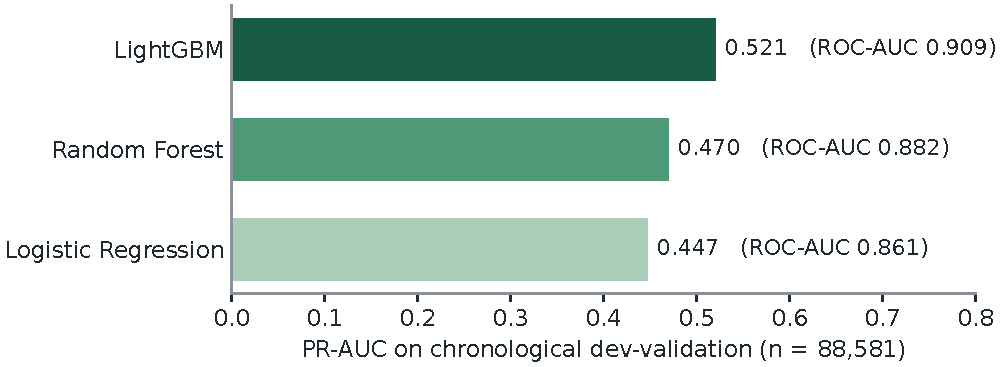
\includegraphics[width=\linewidth]{baselines.pdf}
      \source{Measured on the tuning period (88,581 payments).}
    \column{0.39\textwidth}
      \point{Logistic regression}{A simple weighted sum of the payment details.}
      \vspace{0.5em}
      \point{Random forest}{200 decision trees that vote together.}
      \vspace{0.5em}
      \point{LightGBM}{Trees built one after another, each fixing the previous
        one's mistakes.}
  \end{columns}
  \vfill
  \keyline{\textbf{LightGBM scores 0.521.} Tree models are very strong on table-like data,
    so our deep models must bring something extra.}
\end{frame}

% ---------------------------------------------------------------------
% 12. Transformer results
% ---------------------------------------------------------------------
\speaker{\sAkshin}
\begin{frame}{Transformer results on future payments}
  \vspace{0.6em}
  \begin{columns}[T]
    \column{0.56\textwidth}
      \begin{columns}[T]
        \column{0.48\linewidth}\bignum{0.341}{PR-AUC on the test period\\(about 10$\times$ random guessing)}
        \column{0.48\linewidth}\bignum{27\%}{of fraud caught when only\\1\% of normal payments are flagged}
      \end{columns}
      \vspace{1.4em}
      \point{Fraud changes over time}{During development the score was 0.44; on the newer
        test payments it fell to 0.34. That is why we always test on the future.}
    \column{0.40\textwidth}
      \point{Is the gate stable?}{We trained it 3 times with different random starts:}
      \centering
      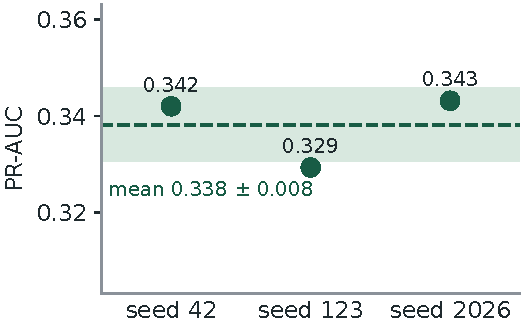
\includegraphics[width=\linewidth]{gate_seeds.pdf}
      \source{Measured on the tuning period.}
  \end{columns}
\end{frame}

% ---------------------------------------------------------------------
% 13. Ablation
% ---------------------------------------------------------------------
\speaker{\sAkshin}
\begin{frame}{Did attention help? An honest experiment}
  \vspace{0.2em}
  \begin{columns}[c]
    \column{0.58\textwidth}
      \centering
      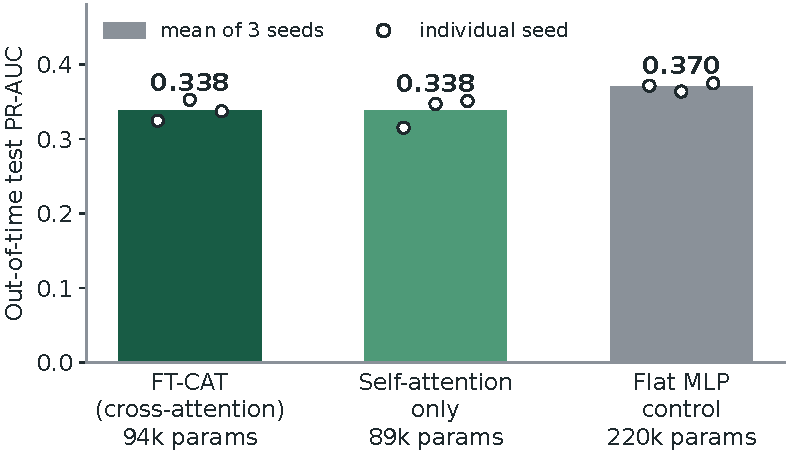
\includegraphics[width=\linewidth]{ablation.pdf}
    \column{0.39\textwidth}
      \point{What we did}{Trained three versions on the same data with the same settings,
        three times each.}
      \vspace{0.5em}
      \point{What we found}{The simple network scored best (0.370); both Transformers
        scored about 0.338.}
      \vspace{0.5em}
      \point{Fair warning}{The simple network had more than twice as many parameters.}
  \end{columns}
  \vfill
  \keyline{Fancier is not automatically better: complex models have to prove they are worth it.}
\end{frame}

% ---------------------------------------------------------------------
% 14. Attention heatmap
% ---------------------------------------------------------------------
\speaker{\sAkshin}
\begin{frame}{Looking inside: where does attention look?}
  \vspace{0.1em}
  \centering
  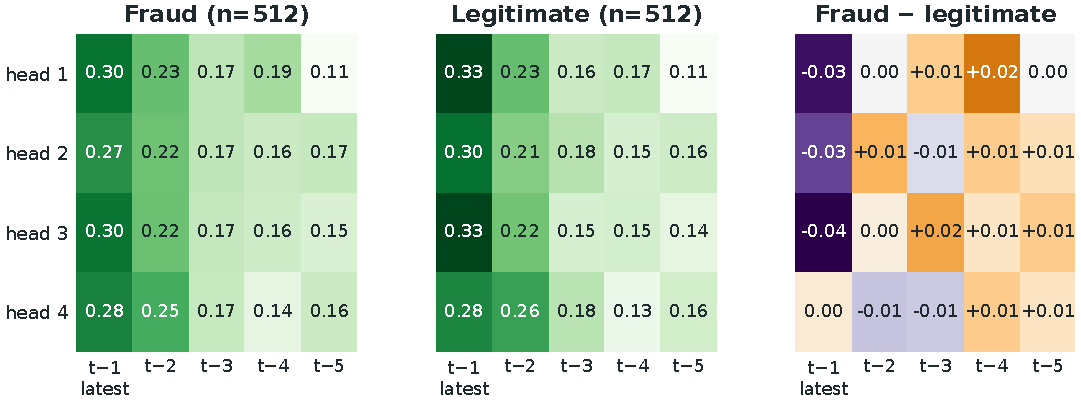
\includegraphics[width=0.72\linewidth]{attention.pdf}
  \raggedright
  \vspace{0.3em}
  \begin{columns}[T]
    \column{0.31\textwidth}
      \point{How to read it}{Each number: how much the model looks at one past payment
        (0.20 = equal attention).}
    \column{0.31\textwidth}
      \point{What we see}{Mostly the latest payment, and almost the same for fraud and
        normal payments.}
    \column{0.31\textwidth}
      \point{What it means}{It is not finding fraud patterns in the history yet; its inputs
        need improving.}
  \end{columns}
\end{frame}

% ---------------------------------------------------------------------
% 15. Focal loss sweep
% ---------------------------------------------------------------------
\speaker{\sAkshin}
\begin{frame}{Tuning the loss: the popular default was not best}
  \vspace{0.1em}
  \centering
  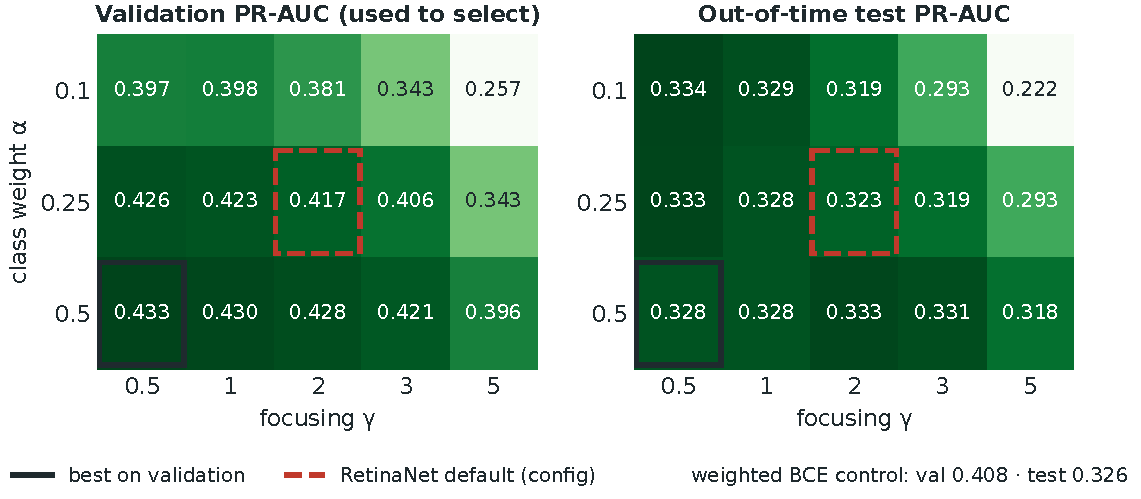
\includegraphics[width=0.62\linewidth]{focal.pdf}
  \raggedright
  \vspace{0.3em}
  \begin{columns}[T]
    \column{0.31\textwidth}
      \point{What we tuned}{Two focal-loss settings: focus on hard examples, and extra
        weight for fraud.}
    \column{0.31\textwidth}
      \point{What we found}{Gentle settings (0.5, 0.5) beat the popular default (2, 0.25);
        very strong focus hurt.}
    \column{0.31\textwidth}
      \point{How big is the effect?}{Small: within about 0.01 of a plain weighted loss
        (one run each).}
  \end{columns}
\end{frame}

% ---------------------------------------------------------------------
% 17. What the autoencoder sees
% ---------------------------------------------------------------------
\speaker{\sSebuhi}
\begin{frame}{What the autoencoder sees}
  \vspace{0.1em}
  \begin{columns}[T]
    \column{0.48\textwidth}
      \centering
      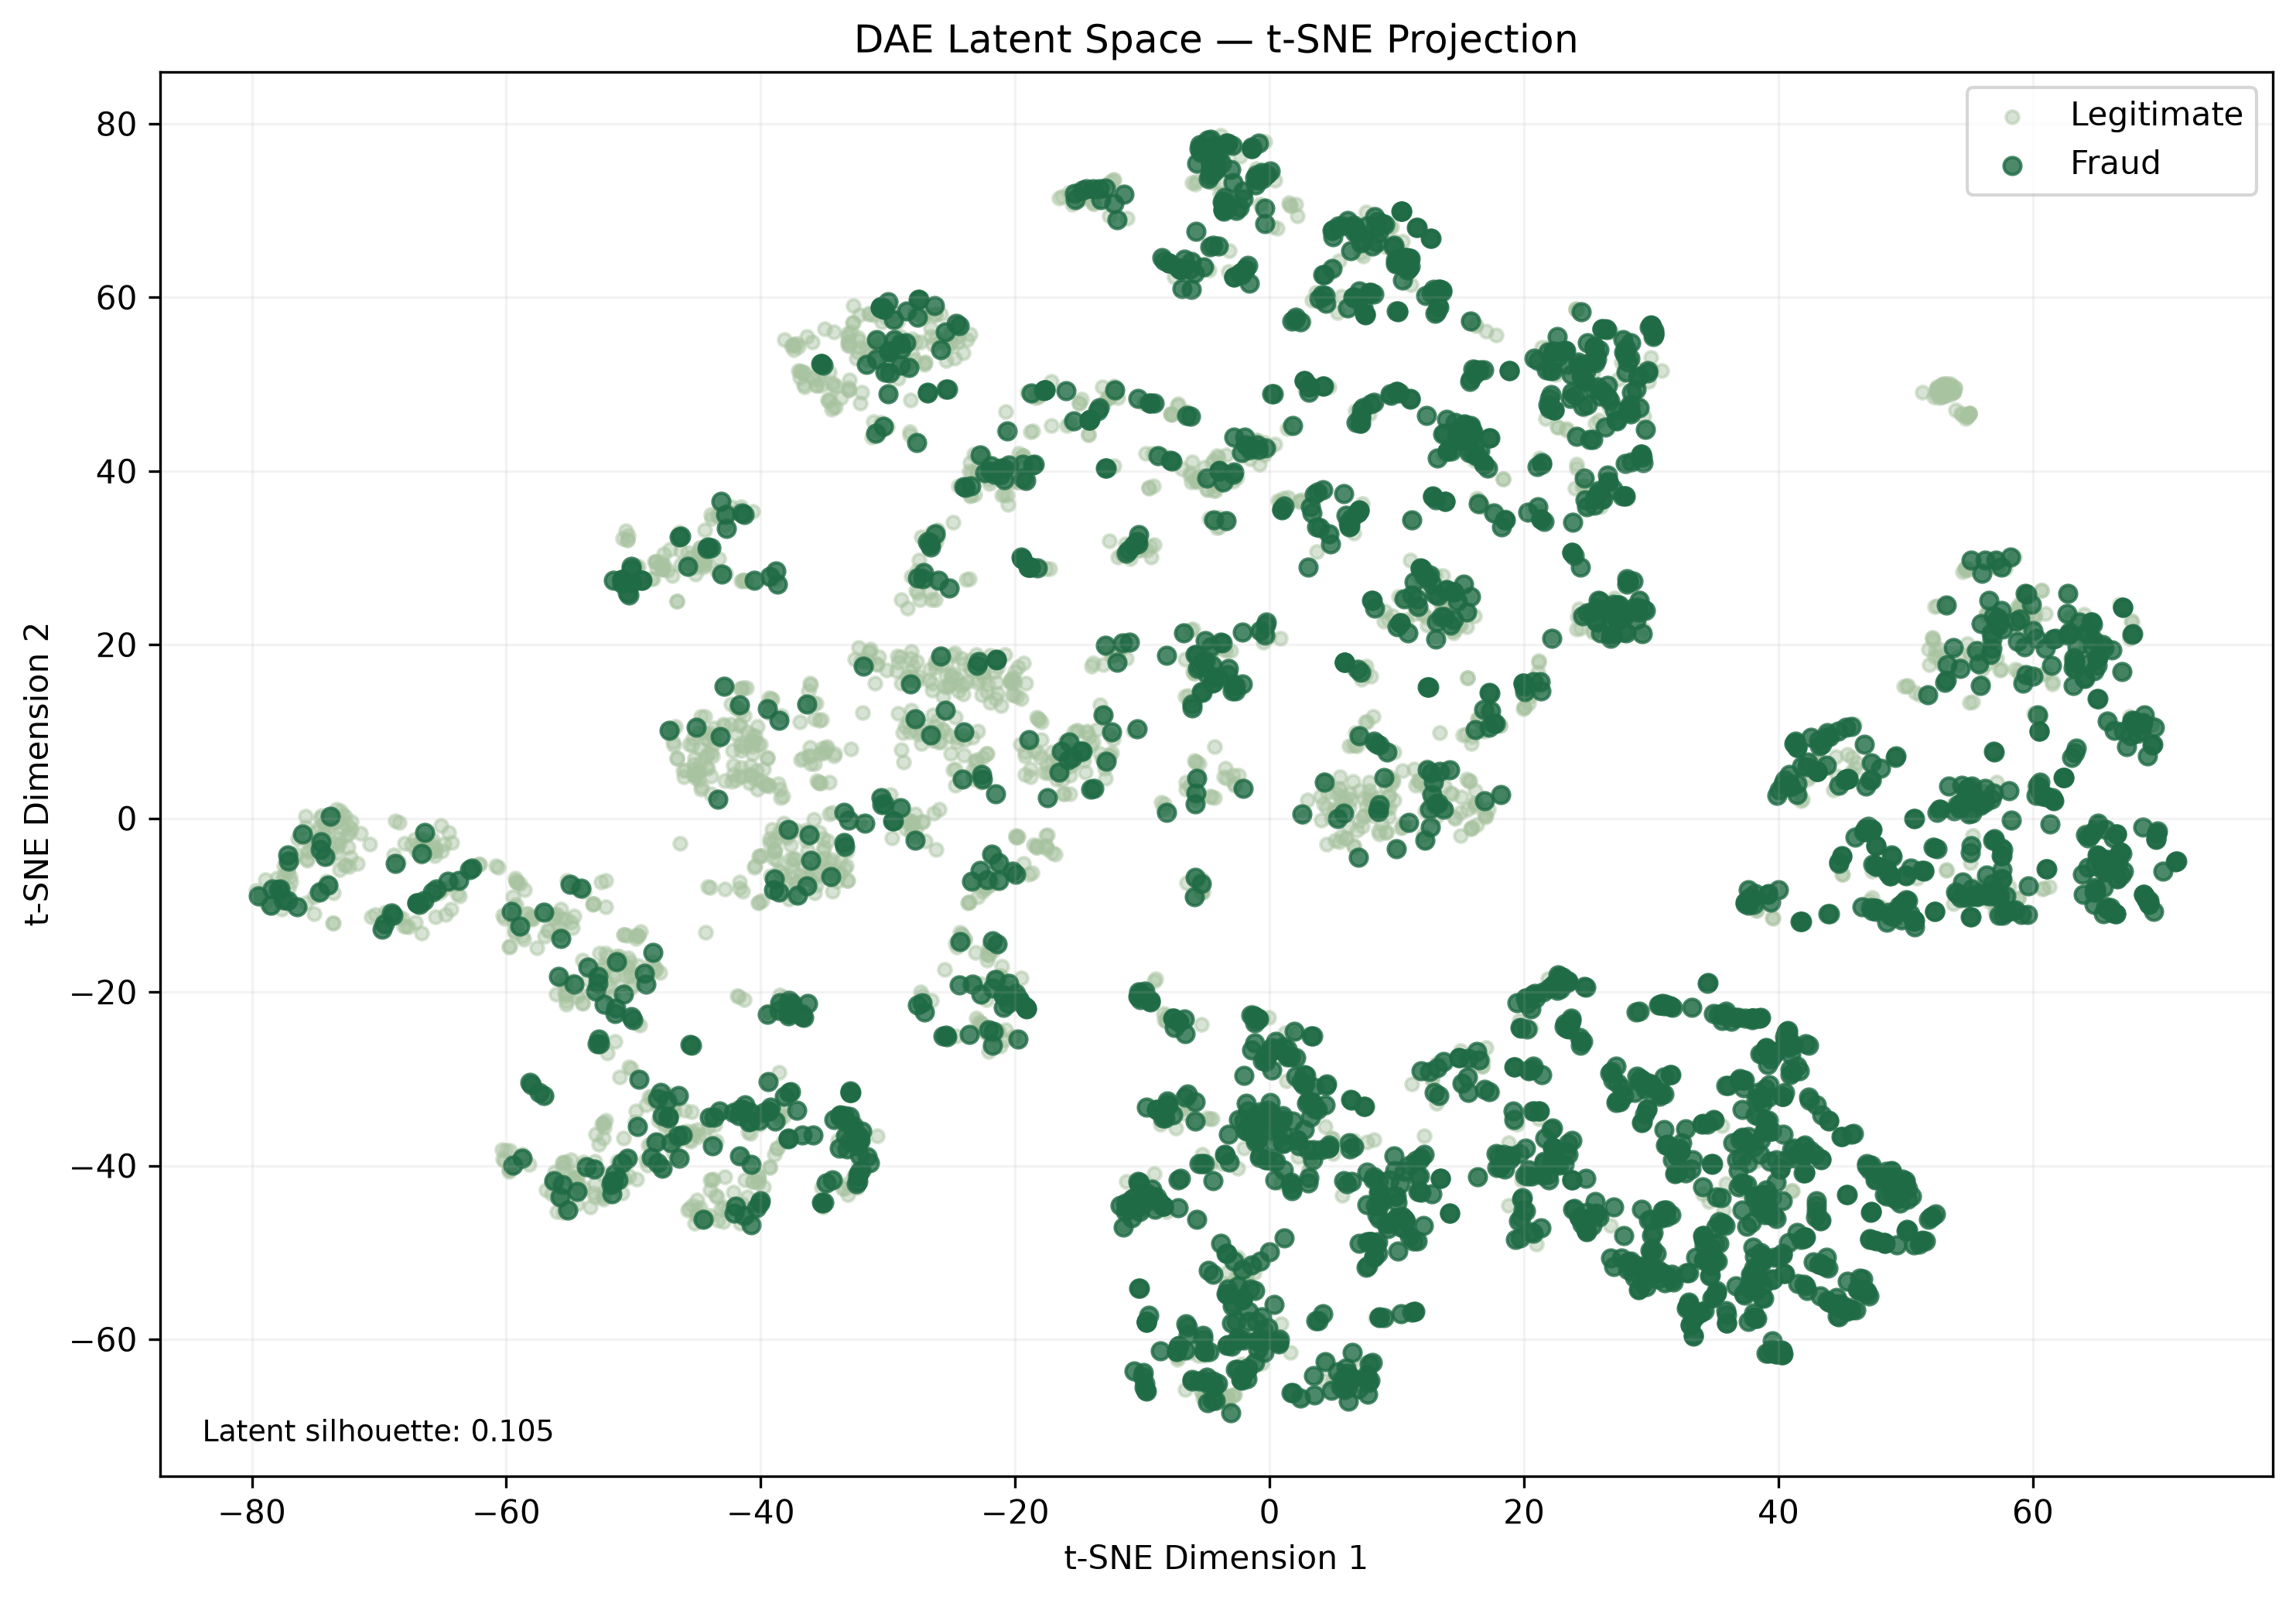
\includegraphics[height=3.7cm]{tsne_latent_space.png}\par
      \vspace{0.25em}
      \raggedright
      \point{A map of its 32 numbers}{Each dot is a payment, flattened to 2D (t-SNE).
        Fraud (dark) and normal (light) overlap, so ``unusual'' does not always mean fraud:
        it helps, but cannot decide alone.}
    \column{0.48\textwidth}
      \centering
      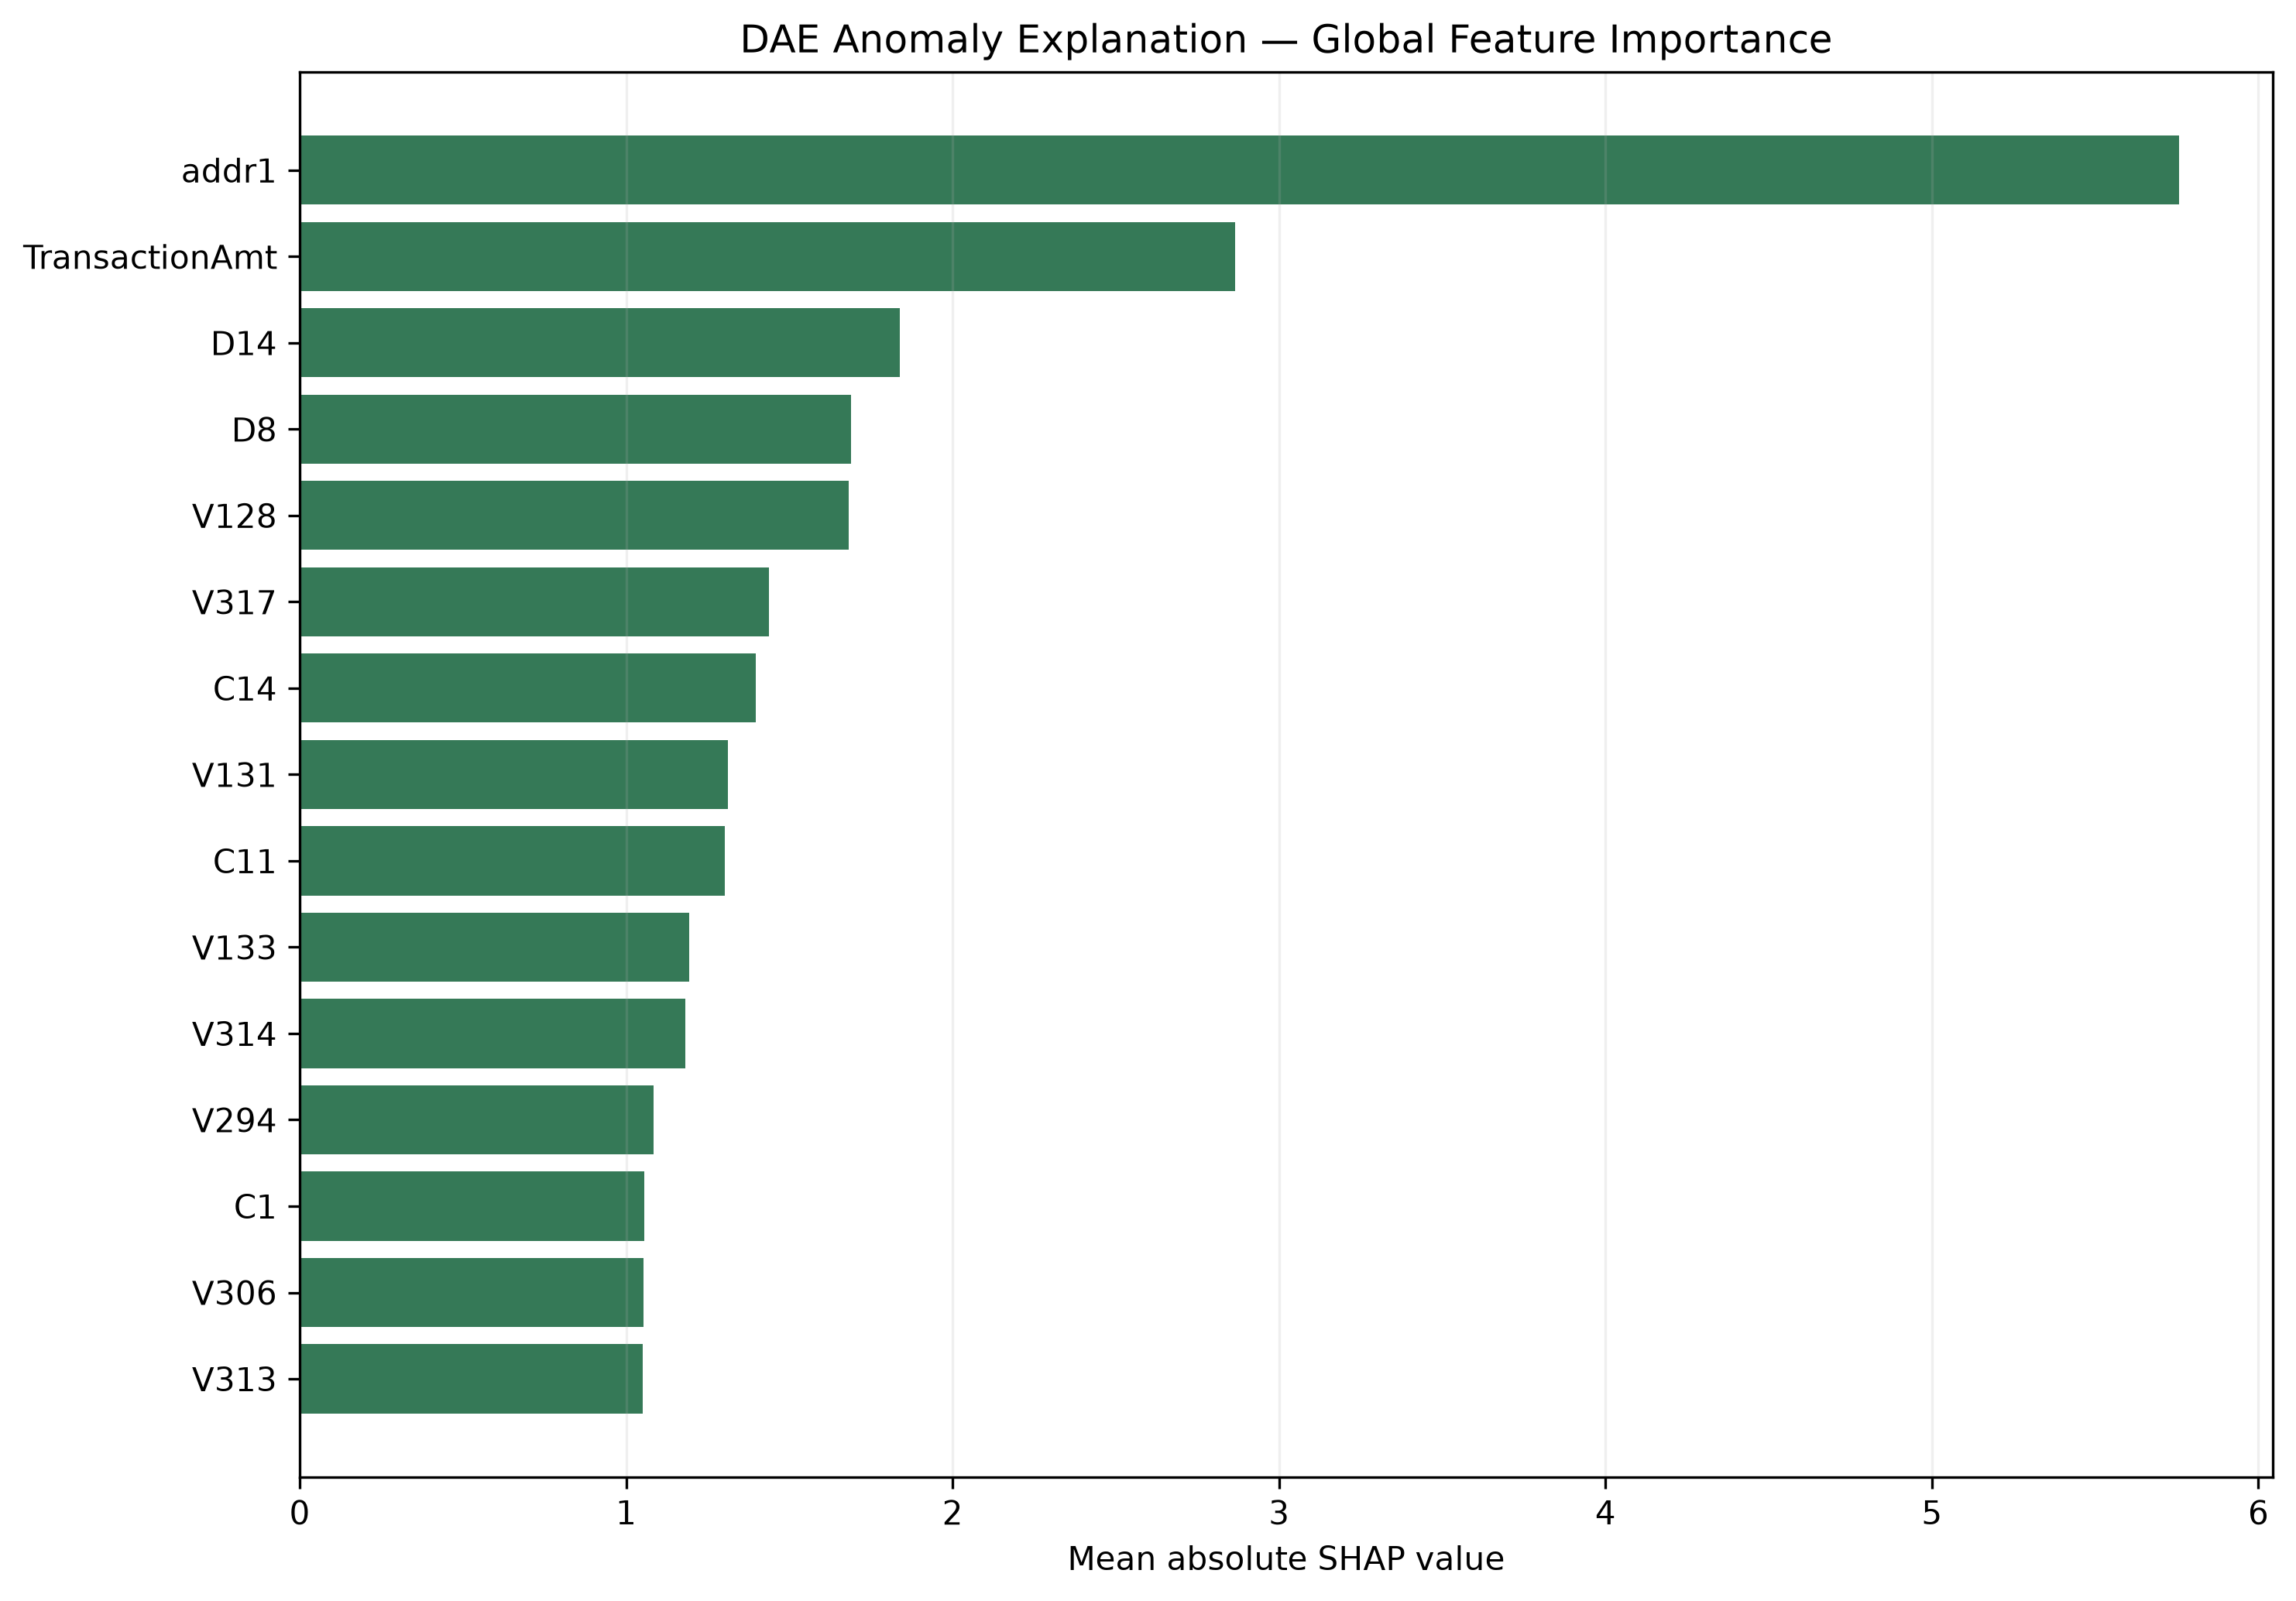
\includegraphics[height=3.7cm]{dae_shap_global_importance.png}\par
      \vspace{0.25em}
      \raggedright
      \point{Which details look unusual?}{SHAP measures how much each detail adds to the
        anomaly score. The address code (\texttt{addr1}) and the amount matter most.}
  \end{columns}
\end{frame}

% ---------------------------------------------------------------------
% 18. Speed
% ---------------------------------------------------------------------
\speaker{\sSebuhi}
\begin{frame}{Fast enough for real-time payments}
  \vspace{0.1em}
  \begin{columns}[T]
    \column{0.24\textwidth}\midnum{6.6 ms}{to score one payment}
    \column{0.24\textwidth}\midnum{2,746}{payments per second}
    \column{0.24\textwidth}\midnum[approve]{CPU only}{no graphics card needed}
    \column{0.24\textwidth}\midnum[muted]{≈2 MB}{autoencoder file size}
  \end{columns}
  \vspace{0.3em}
  \centering
  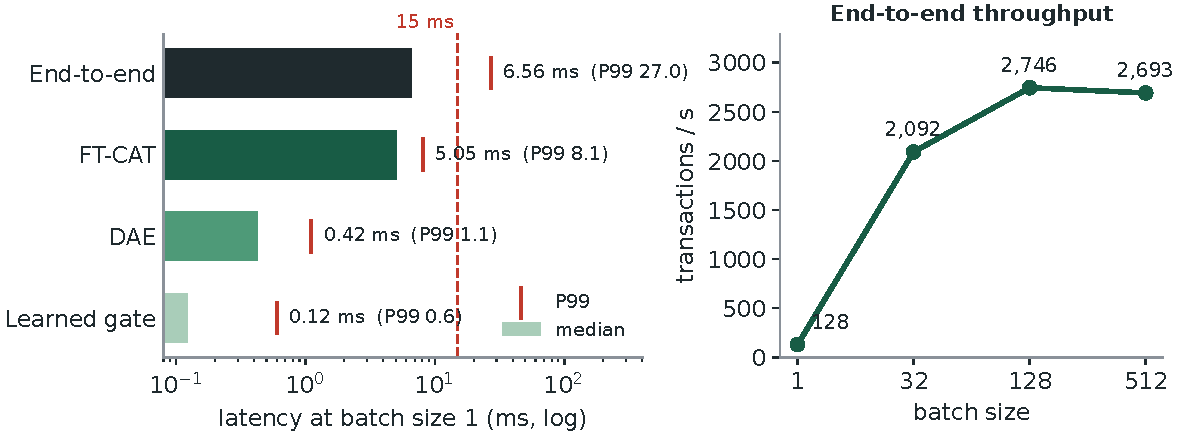
\includegraphics[height=2.95cm]{latency.pdf}
  \raggedright
  \keyline{The Transformer takes most of the time. Typical: 6.6 ms; the slowest 1 in 100 take
    27 ms or more (goal: 15 ms).}
  \source{Measured on a single-CPU machine; model time only, without network overhead.}
\end{frame}

% ---------------------------------------------------------------------
% 19. Product
% ---------------------------------------------------------------------
\speaker{\sHabil}
\begin{frame}{The product: a dashboard for fraud analysts}
  \vspace{0.2em}
  \begin{columns}[T]
    \column{0.62\textwidth}
      \centering
      \screenshot{dashboard_prediction.png}{\linewidth}{Prediction page screenshot}\par
      \vspace{0.15em}
      {\scriptsize\color{muted}A real test payment is scored and sent to human review}%
      \hfill\chip{brand}{LIVE DEMO $\rightarrow$}
    \column{0.35\textwidth}
      \centering
      \screenshot{dashboard_command.png}{0.8\linewidth}{Command page screenshot}\par
      {\scriptsize\color{muted}System status}\par
      \vspace{0.25em}
      \screenshot{dashboard_conformal.png}{0.8\linewidth}{Conformal Triage screenshot}\par
      {\scriptsize\color{muted}Confidence check results}
  \end{columns}
\end{frame}

% =====================================================================
\section{Wrap-up}
% =====================================================================

% ---------------------------------------------------------------------
% 21. Conclusion
% ---------------------------------------------------------------------
\speaker{\sHabil}
\begin{frame}{Conclusion}
  \vspace{0.4em}
  \begin{columns}[T]
    \column{0.31\textwidth}
      \begin{beamercolorbox}[wd=\linewidth,sep=0.55em,rounded=true]{card}
        {\small\bfseries\color{brand}Decisions, not just scores\par}\vspace{0.3em}
        {\footnotesize 76.8\% of payments are approved automatically; humans review
        23.2\% and see 71\% of all fraud.\par}
      \end{beamercolorbox}
    \column{0.31\textwidth}
      \begin{beamercolorbox}[wd=\linewidth,sep=0.55em,rounded=true]{card}
        {\small\bfseries\color{brand}Honestly tested\par}\vspace{0.3em}
        {\footnotesize Two detectors combined by a gate, tested on future payments, and
        we show the results that did not go our way.\par}
      \end{beamercolorbox}
    \column{0.31\textwidth}
      \begin{beamercolorbox}[wd=\linewidth,sep=0.55em,rounded=true]{card}
        {\small\bfseries\color{brand}Ready to run\par}\vspace{0.3em}
        {\footnotesize 6.6 ms per payment on a normal CPU, with a web API and an analyst
        dashboard.\par}
      \end{beamercolorbox}
  \end{columns}
  \vspace{0.8em}
  \small\textbf{\color{brand}Next steps}\par
  \vspace{0.3em}
  \begin{columns}[T]
    \column{0.48\textwidth}
      \footnotesize
      \begin{itemize}\setlength{\itemsep}{0.2em}
        \item Separate safety targets for fraud and for normal payments
        \item Watch for changing fraud patterns and recalibrate regularly
      \end{itemize}
    \column{0.48\textwidth}
      \footnotesize
      \begin{itemize}\setlength{\itemsep}{0.2em}
        \item Explain the final decision, not just one part
        \item Find a safe setting that allows automatic blocking
      \end{itemize}
  \end{columns}
\end{frame}

% ---------------------------------------------------------------------
% 22. Questions
% ---------------------------------------------------------------------
{
\setbeamertemplate{footline}{}
\begin{frame}[plain]
  \begin{tikzpicture}[remember picture,overlay]
    \fill[brand] (current page.north west) rectangle ([xshift=0.42cm]current page.south west);
  \end{tikzpicture}
  \vfill
  \centering
  {\fontsize{30}{34}\selectfont\bfseries\color{brand}Thank you}\par
  \vspace{0.4em}
  {\Large\color{ink}Questions?}\par
  \vspace{1.2em}
  \chip{approve}{APPROVE}\ \chip{review}{REVIEW}\ \chip{block}{BLOCK}\par
  \vspace{1.2em}
  {\footnotesize\color{muted}github.com/sa6uhi/DL-final-project\enspace\textperiodcentered\enspace
    report: report/report.pdf}\par
  \vspace{0.4em}
  {\footnotesize \sNadir\enspace\textperiodcentered\enspace \sAkshin\enspace\textperiodcentered\enspace
    \sHabil\enspace\textperiodcentered\enspace \sSebuhi}\par
  \vfill
\end{frame}
}

\end{document}
